\newcommand{\ClassPath}{../../VIU_TFM_LaTeX_template}
\documentclass{\ClassPath/viu-tfm-template}
\usepackage{multicol}

\definecolor{maincolor}{HTML}{f25416}

%--------------------------------------------------------------------------
% Definiciones necesarias Modifica con tus datos
%--------------------------------------------------------------------------
\def\nombre{Gómez Olivencia, Rubén}
\def\dni{78910013-A}
\def\titulo{Biblioteca de series en PHP}
\def\titulacion{Máster Universitario en Desarrollo de Aplicaciones y Servicios Web}
\def\curso{2022-2023}

%Los siguientes son opcionales: si no se ponen, la portada cambia un poco. Ideal para escribir artículos/trabajos cortos
\def\dirige{}
\def\convocatoria{}
\def\asignatura{Desarrollo de aplicaciones web I: Lado del servidor (\textit{back-end})}


% importar fichero de Bibliografía
%\addbibresource{Actividad_1.bib}

\begin{document}
\graphicspath{{../../VIU_TFM_LaTeX_template/}}

\coverpage

\tableofcontents

\chapter{Introducción}

A lo largo de este documento se van a explicar las decisiones tomadas, tanto en el ámbito de programación como de diseño, durante el desarrollo de una aplicación web para gestionar una biblioteca que contiene series, sus episodios y los actores que aparecen en ellos.

Para la realización de esta web se ha hecho uso del lenguaje de programación \href{https://www.php.net/}{PHP} para la parte \textit{\textbf{back-end}}, junto con \textbf{javascript} para la programación \textbf{\textit{front-end}}.


\chapter{Requisitos del proyecto}

Como todo proyecto, existen unos requisitos que deben ser cumplidos al terminar el desarrollo. De manera resumida, los requisitos son los siguientes:

\vspace{-1em}
\begin{itemize}
    \item Biblioteca de series con 5 tablas (plataforms de emisión, series, actores, directores, idiomas y series).
    \item Uso del patrón \textbf{MVC} (Modelo - Vista - Controlador) a la hora     de programar.
    \item Al menos tres vistas para cada entidad
\end{itemize}
\vspace{-1em}

Como se verá a continuación, todos los requisitos se han cumplimentando, tras realizar una pequeña modificación al modelo de datos.

\chapter{Modelo de datos}
A la hora de gestionar una biblioteca de series, hay que tener en cuenta que estas cuentan con episodios, por lo que se ha añadido esta nueva entidad.

Por otro lado, dado que actor y director pueden ser el mismo, y aparte, puede haber mucha más gente involucrada en una serie, por lo tanto se ha decidido unificar dichas entidades en una, para después gestionar el papel que realizan por cada episodio.

El esquema \textbf{Entidad - Relación} final queda de la siguiente forma:

\begin{center}
    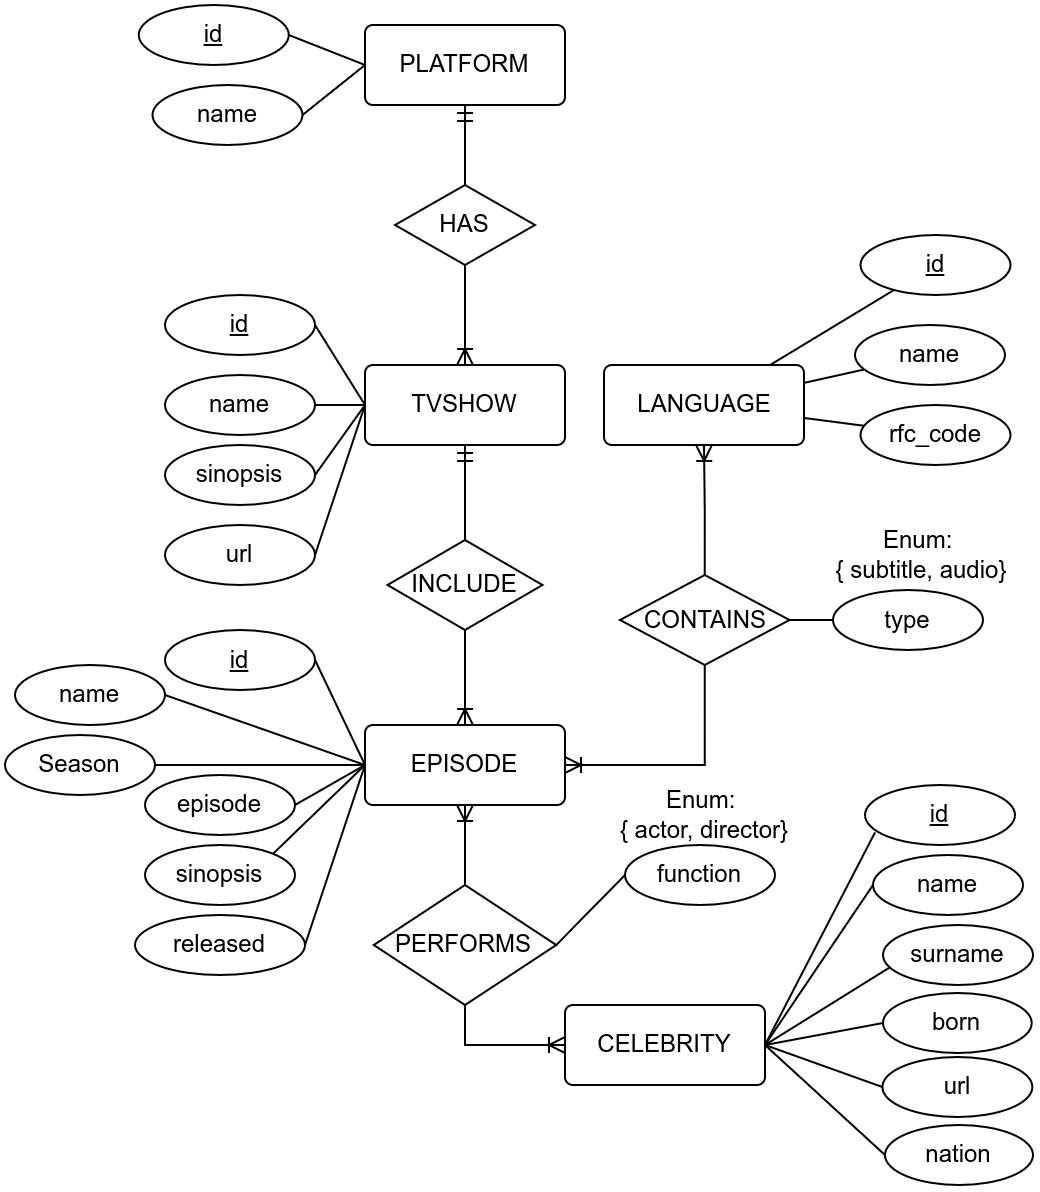
\includegraphics[width=0.8\linewidth]{img/entidad-relacion.png}
\end{center}


Este esquema entidad-relación ha dado lugar a un total de siete tablas cuyo esquema físico se puede importar desde el fichero \configfile{create_schema.sql} a MySQL, tal como veremos más adelante.

\chapter{Despliegue de la aplicación}
Antes de entrar en detalle en cómo se ha desarrollado la aplicación es importante conocer cómo podemos realizar el despliegue de la aplicación, ya sea para utilizarla o para realizar modificaciones sobre la misma.

\section{Servicios Docker}
Para realizar el desarrollo del proyecto se ha utilizado servicios a través de contenedores \textbf{\href{https://www.docker.com/}{Docker}}, los cuáles pueden ser levantados gracias al fichero \configfile{compose.yaml} y el comando \commandbox{docker-compose up}
.


\begin{mycode}{Parte del fichero \textbf{compose.yaml}}{yaml}{}
services:
    php:
        image: docker.io/webdevops/php-nginx-dev:8.1
        ports:
            - '80:80'
        environment:
            - PHP_DISPLAY_ERRORS=1
            - PHP_DATE_TIMEZONE="Europe/Madrid"
        volumes:
            - './src:/app'
        depends_on:
            - mysql
...
\end{mycode}

Este fichero se encarga de desplegar los siguientes \textit{containers}:
\vspace{-1em}
\begin{enumerate}
    \item \textbf{PHP+Nginx}: Servicio de backend con el servidor web
    \href{https://nginx.org/}{Nginx} y el servicio \href{https://php-fpm.org/}{PHP-FPM} para realizar el procesado de PHP.
    \item \textbf{MySQL}: Servidor de base de datos relacional donde irán los datos.
    \item \textbf{PHPMyAdmin}: Para gestionar de manera más sencilla la base de datos.
\end{enumerate}
\vspace{-1em}

Al levantar los servicios con el comando \textbf{docker-compose up} se hará uso de los siguientes puertos:
\vspace{-1em}
\begin{itemize}
    \item \textbf{80}: Para el entorno web.
    \item \textbf{3306}: Para la base de datos.
    \item \textbf{3307}: Para phpmyadmin.
\end{itemize}
\vspace{-1em}

\section{Despliegue del código fuente}
Para realizar el despliegue del código fuente sobre el contenedor de \textbf{PHP}, el directorio \configdir{src} debe estar situado a la misma altura del fichero \configfile{compose.yaml}.

De esta manera, a la hora de levantar el servicio se crea un volumen compartiendo el directorio local \configdir{src} con otro dentro del contenedor, en la ruta \configdir{/app}, que es de donde se nutre Nginx.


\section{Creación de la base de datos}

El servicio de MySQL se encarga de crear una base de datos llamada \textbf{actividad1} en el momento en el que el servicio se levanta. También crea los siguientes credenciales de acceso a dicha base de datos:

\vspace{-1em}
\begin{itemize}
    \item usuario:  \textbf{actividad1}
    \item contraseña:  \textbf{4ct1v1d4d1}
\end{itemize}
\vspace{-1em}

\section{Despliegue de datos}
Para realizar el despliegue de datos, vamos a hacer uso de los siguientes ficheros que acompañan esta memoria y el código fuente:

\vspace{-1em}
\begin{itemize}
    \item \configfile{create_schema_con_inserts.sql}: Para crear las tablas con datos reales que pueden ser utilizados junto con la aplicación. \textbf{Se recomienda usar este fichero}.
    \item \configfile{create_schema.sql}: Para realizar la creación de las tablas necesarias para el proyecto. No existen datos.
\end{itemize}
\vspace{-1em}

Estos ficheros se pueden importar a través del servicio \textbf{PHPMyAdmin} comentado previamente, a través de un navegador web y el puerto 3307.


\chapter{Desarrollo realizado}

Una vez tenemos realizado el despliegue, se va a profundizar en el desarrollo realizado, destacando los siguientes aspectos:

\section{Configuración de la aplicación}
Aunque la aplicación realizada es sencilla, para evitar tener que estar repitiendo código, y buscando facilitar una futuro expansión del proyecto, se ha creado un fichero de configuración \configfile{config.php}.

Este fichero actualmente cuenta con una variable \inlineconsole{$conf}, que es un array, que cuenta con distintas posiciones en las que podemos diferenciar tres tipos de configuraciones:
\vspace{-1em}
\begin{itemize}
    \item \textbf{Nombre de la aplicación}: De esta manera, podemos reutilizar el código de la aplicación, y creando de manera sencilla distintas instancias de la misma.
    \item \textbf{Acceso a base de datos}: Para configurar el acceso a base de datos tenemos las opciones: servidor, puerto, usuario, contraseña y nombre de la base de datos. \textbf{Estas opciones deben ser configuradas para el servidor correspondiente}.
    \item \textbf{Rutas}: Para configurar dónde se van a guardar las imágenes subidas a través de la aplicación.
\end{itemize}
\vspace{-1em}

\section{Modelo MVC}
Uno de los requisitos era hacer uso del modelo Modelo-Vista-Controlador (\textbf{MVC}), a la hora de programar. Es por ello que dentro del directorio entregado con el código fuente existen tres directorios principales dedicados a este modelo de programación:

\vspace{-1em}
\begin{itemize}
    \item \configdir{models} Dentro de este directorio se encuentran los distintos modelos de datos que se utilizan dentro de la aplicación web. Estos modelos son creados a través de clases en PHP, que generan objetos. Debido al modelo relacional creado, algunas de las clases contienen como atributos otros objetos.

    Por ejemplo, un episodio tiene como atributo (a través de un identificador propio) la serie a la que pertenece, realizando de esta manera programación orientada a objetos, y a través de un episodio poder acceder a su elemento padre.

    \item \configdir{controllers} En este directorio se encuentran distintos ficheros, uno por cada modelo existente, que contienen distintas funciones para ser el nexo de unión entre los modelos de datos y las vistas. En este directorio se quieren destacar dos ficheros “especiales”:
    \begin{itemize}
        \item \textbf{DB.php}: Este fichero contiene funciones que tienen que ver con la base de datos. Principalmente la gestión de la conexión a MySQL y el uso de una función genérica que recibe una \textit{query}, la ejecuta y devuelve los valores. De esta manera se ha tratado de buscar la eficiencia y el no repetir código fuente a lo largo de la aplicación.

        \item \textbf{helpers.php}: Este es un fichero que contiene distintas funciones que pueden ser utilizadas a lo largo de toda la aplicación, y que no tienen que ver con un modelo concreto de datos.

        El ejemplo más claro es la función llamada “\textbf{getAlert}”, que dependiendo de los parámetros recibidos devolverá un aviso de éxito o de error.

        Otras funciones de este fichero son “\textbf{changeDateFormat}” para el cambio de fecha a formato en castellano o el guardado de imágenes.

        La creación de este fichero se ha basado en el \textit{framework} \textbf{Ruby On Rails}, el cual cuenta con unos ficheros “\_helpers.rb” cuya función es similar, y buscando la \textbf{no duplicación de código fuente}.
    \end{itemize}

    \item \configdir{views} Directorio que contiene las vistas creadas para cada uno de los modelos, separados por directorios. En el siguiente punto se va a detallar más sobre este aspecto.
\end{itemize}

\section{Creación de “plantillas” para las vistas}
Dado que en una aplicación web existe la posibilidad de mostrar información relacionada desde distintos apartados, se ha tratado de evitar la duplicación de código en la medida de lo posible creando un sistema de “plantillas” propio.

Vamos a poner un ejemplo sencillo, la \textbf{creación y edición de un episodio}. Para crearla, se mostrará un  formulario con una serie de campos (nombre, apellido, fecha de emisión, ...) que deben ser rellenados antes de guardar la información.

A la hora de editar, se necesita un formulario que muestre la información para que pueda ser modificada. Es por eso, que en lugar de crear dos formularios en dos ficheros distintos, se ha creado un fichero \configfile{_form.php} que contiene el formulario y es importado desde sus correspondientes ficheros: \configfile{new.php} y \configfile{edit.php}

Este uso de plantillas no sólo se ha limitado a los formularios, ya que también se ha utilizado para ciertos listados que muestran los mismos datos pero desde distintas páginas:
\begin{center}
    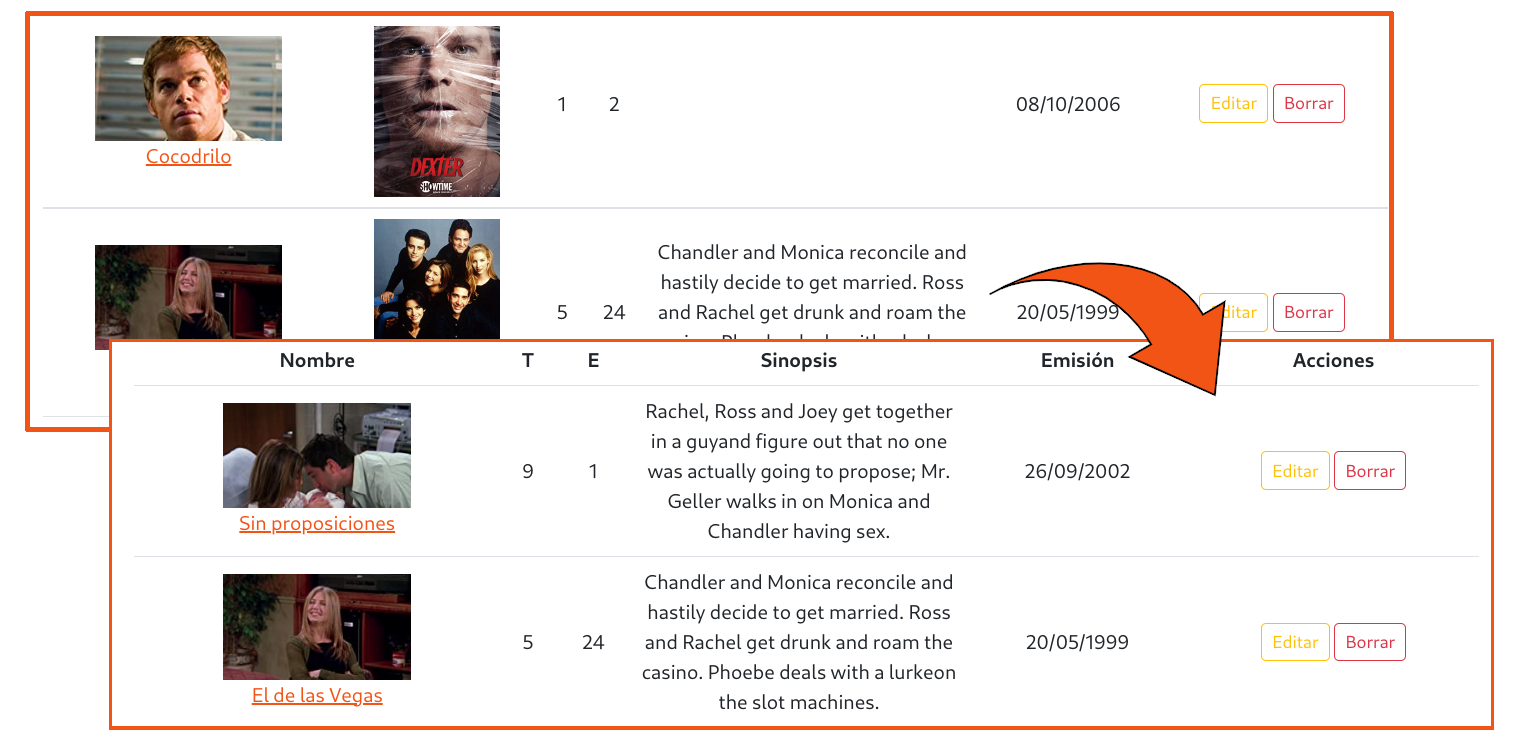
\includegraphics[width=0.8\linewidth]{img/vistas.png}
\end{center}
\vspace{-1em}

Tal como se puede ver en la imagen, existen dos listados que muestran episodios de series, pero que se visualizan en distintos sitios de la aplicación web (el listado general de episodios, y al ver una serie concreta).

El ejemplo muestra por un lado todos los episodios guardados en la base de datos (a través de este \href{http://localhost/views/episodes/}{enlace local}), y por otro los episodios de la serie “Friends” (a través de este \href{http://localhost/views/tvshows/show.php?id=4}{enlace local}), que utiliza como fichero de plantilla  \configfile{views/episodes/_list.php} que es incluido a través de la sentencia \inlineconsole{include_once("../episodes/_list.php");} desde la vista \configfile{views/tvshows/show.php}.

En este caso, en la vista existe cierta programación para que teniendo en cuenta cuál es el origen de la visualización, se muestren más columnas o menos.

Este sistema de plantillas es habitual en todo tipo de frameworks, que permiten aislar de mejor manera distintas secciones, e incluso permiten el paso de parámetros. En este caso se ha realizado de manera “más artesanal”, pero consiguiendo la finalidad, que es la no duplicidad de código.

\section{Carga de imágenes a través de los formularios}
Para mejorar el aspecto visual y la información que se puede guardar de las series y los episodios, se ha añadido la posibilidad de subir imágenes.

De esta manera, las plataformas, series, episodios y \textit{celebrities} podrán contar con una imagen asociada mejorando el aspecto de toda la web, como acompañante a la información.

\begin{center}
    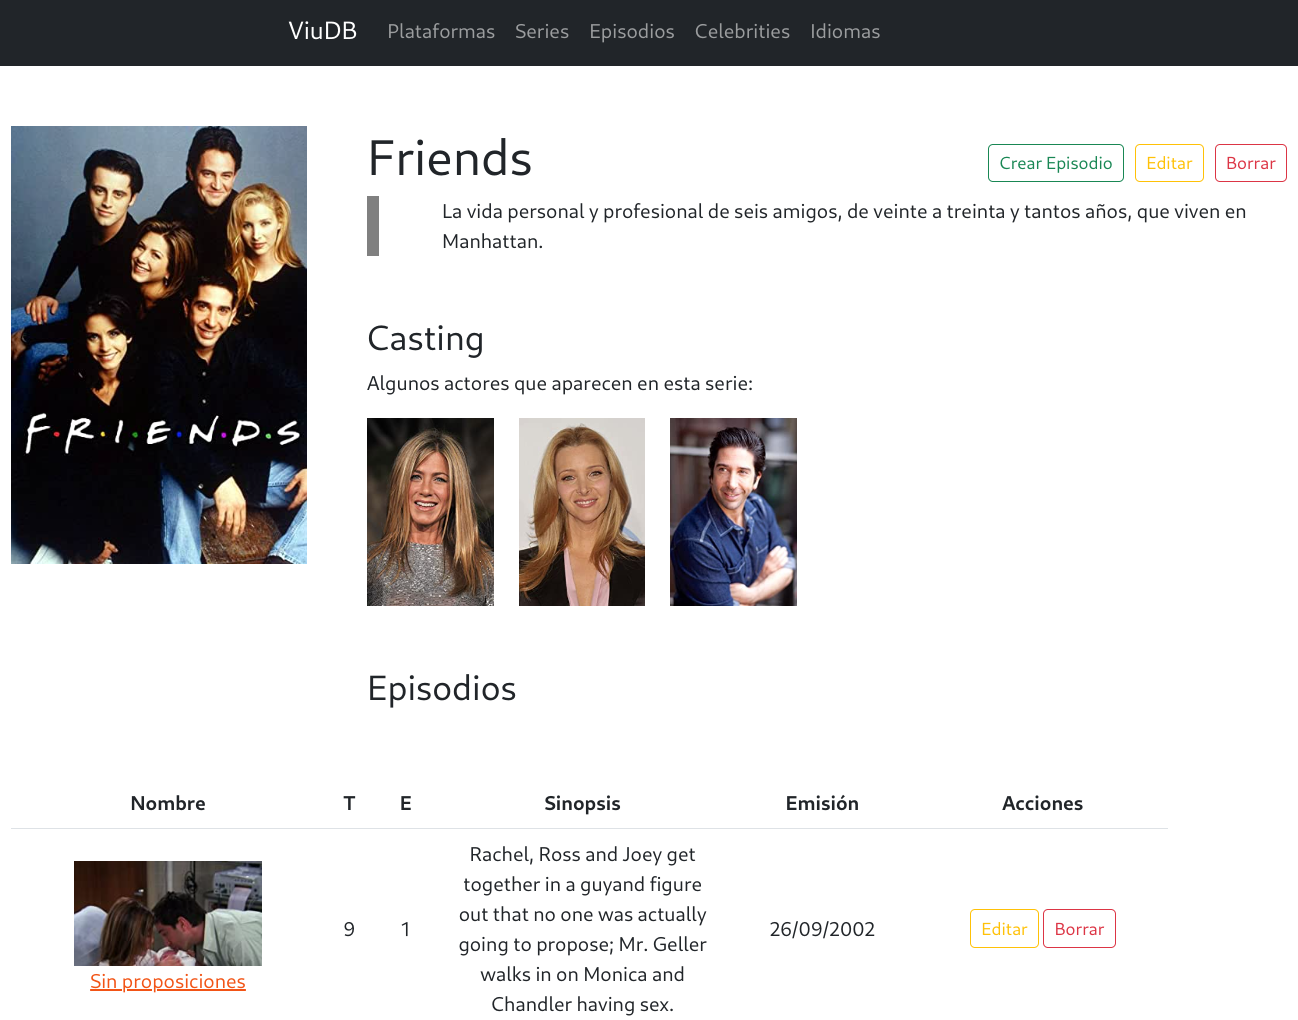
\includegraphics[frame,width=0.75\linewidth]{img/general.png}
\end{center}
\vspace{-1.5em}

Tal como se puede ver en la imagen, el uso de imágenes hace que la información que aparece en la web resulte más atractiva al usuario.

\section{Uso de javascript para llamadas asíncronas}
Para obtener información sin necesidad de acceder a una página web, y para realizarlo de manera asíncrona, se ha hecho uso de peticiones \textit{\textbf{fetch}} a través del lenguaje \textbf{Javascript}.

Las funciones javascript que se han creado están en el fichero \configfile{assets/js/viudb.js} y son llamadas desde algunos de los botones “borrar” que aparecen en la web.

Por ejemplo, si queremos borrar una serie, se realiza una petición consultando el número de episodios que tiene esa serie para terminar mostrando esa información en un “modal” de confirmación.

\vspace{-1em}
\begin{center}
    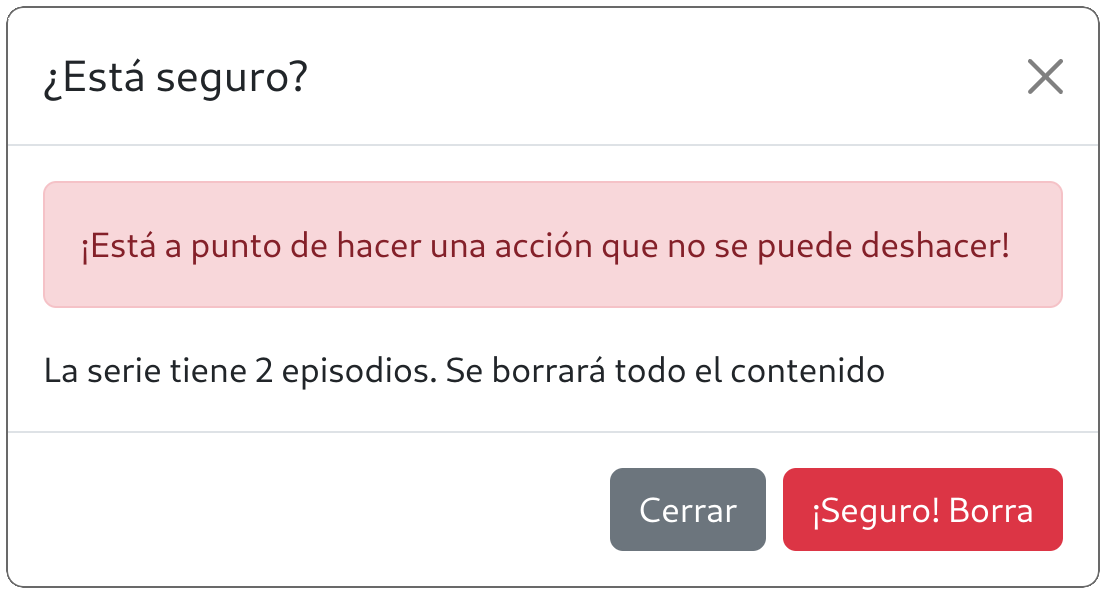
\includegraphics[width=0.5\linewidth]{img/modal.png}
\end{center}
\vspace{-1.5em}


\chapter{Dificultades del proyecto}

Como todo proyecto de programación, durante el desarrollo nos podemos encontrar con ciertas dificultades que deben ser subsanadas para llegar a cumplir los requisitos planteados al comienzo del proyecto.

En este caso, al ser la primera vez por parte del programador en llevar a cabo una aplicación web en \textbf{PHP}, ha habido distintos aspectos que han sido tratados por primera vez, pero que se han podido equiparar a otros proyectos con otros lenguajes. Por ejemplo:

\vspace{-1em}
\begin{itemize}
    \item \textbf{Gestión de consultas a base de datos}: Ha sido interesante conocer cómo se gestionan las consultas a base de datos a través de la librería \textbf{mysqli}, y las distintas maneras de obtener los resultados obtenidos.
    \item \textbf{Consulta de errores producidos}: Ha habido que configurar el contenedor Docker con la variable de entorno \textbf{PHP\_DISPLAY\_ERRORS=1} para que se muestren los errores producidos durante el desarrollo.
    \item \textbf{Gestión de validación “a mano”}: Al no haber podido contar con un \textit{framework}, la validación de la información obtenida de los formularios se ha realizado de manera manual, lo que dificulta el proceso, pero a la vez se aprende de la importancia del proceso.
\end{itemize}


\chapter{Mejoras a realizar}
Como todo proyecto, y más cuando se realiza en un tiempo limitado, existen distintos aspectos que se pueden mejorar pero que son relegados para terminar en tiempo y forma. A continuación se detallan algunas posibles mejoras:

\vspace{-1em}
\begin{itemize}
    \item \textbf{Frameworks}: El uso de frameworks de programación permite la simplificación de código a distintos niveles dentro de una aplicación web.
    \item \textbf{\textit{Scrapper} de imágenes e información}: Sería interesante que en lugar de pedirle toda la información de una serie al usuario, que sólo indicase la URL de \href{https://www.imdb.com/}{IMDB} de la serie, y a través de un proceso en el \textbf{\textit{backend}} se obtuviese toda la información (sinopsis, capítulos, actores, portada de la serie...) de manera automática.
\end{itemize}


\chapter{Conclusiones}

A la hora de desarrollar una aplicación web es importante conocer cómo se gestiona la información en el lado de servidor. Este proyecto ha permitido profundizar en diferentes ámbitos utilizados en el desarrollo \textbf{back-end} como son: el patrón \textbf{MVC}, la validación de datos obtenidos en peticiones, gestión a base de datos, ...

Por otro lado, es importante conocer el lenguaje de programación que se va a utilizar antes de afrontar un proyecto. Y aunque no se tenía demasiada experiencia con el lenguaje \textbf{PHP}, este no ha dado problemas durante el desarrollo. Aunque es cierto que se ha notado la ausencia del uso de un \textit{framework} que facilite ciertas tareas durante el proceso.

\end{document}
